% Template of basic phisics experiment 基于 article template, 在此基础上做修改
% 设定文章编码类型, 正文字号为五号则 zihao=5, 正文字号为小四则 zihao=-4
\documentclass[zihao=5, UTF8]{article}		


% 自定义宏定义
\def\N{\mathbb{N}}
\def\F{\mathbb{F}}
\def\Z{\mathbb{Z}}
\def\Q{\mathbb{Q}}
\def\R{\mathbb{R}}
\def\C{\mathbb{C}}
\def\T{\mathbb{T}}
\def\S{\mathbb{S}}
\def\A{\mathbb{A}}
\def\I{\mathscr{I}}
\def\d{\mathrm{d}}
\def\p{\partial}


% 物理实验报告所需的其它宏包
\usepackage{ulem}   % \uline 下划线支持

% 导入基本宏包
\usepackage[UTF8]{ctex}     % 设置文档为中文语言
\usepackage[colorlinks, linkcolor=blue, anchorcolor=blue, citecolor=blue, urlcolor=blue]{hyperref}  % 宏包: 自动生成超链接 (此宏包与标题中的数学环境冲突)
% \usepackage{docmute}    % 宏包: 子文件导入时自动去除导言区, 用于主/子文件的写作方式, \include{./51单片机笔记}即可. 注: 启用此宏包会导致.tex文件capacity受限. 
\usepackage{amsmath}    % 宏包: 数学公式
\usepackage{physics}
\usepackage{bm}
\usepackage{mathrsfs}   % 宏包: 提供更多数学符号
\usepackage{amssymb}    % 宏包: 提供更多数学符号
\usepackage{pifont}     % 宏包: 提供了特殊符号和字体
\usepackage{extarrows}  % 宏包: 更多箭头符号
\usepackage{multirow}
\usepackage{siunitx}

\renewcommand{\dd}{\mathrm{d}}

% 列表环境设置
\usepackage{enumitem}   % 宏包: 列表环境设置
    \setlist[enumerate]{itemsep=0pt, parsep=0pt, topsep=0pt, partopsep=0pt, leftmargin=3.5em} 
    \setlist[itemize]{itemsep=0pt, parsep=0pt, topsep=0pt, partopsep=0pt, leftmargin=3.5em}
    \newlist{circledenum}{enumerate}{1} % 创建一个新的枚举环境  
    \setlist[circledenum,1]{  
        label=\protect\circled{\arabic*}, % 使用 \arabic* 来获取当前枚举计数器的值, 并用 \circled 包装它  
        ref=\arabic*, % 如果需要引用列表项, 这将决定引用格式(这里仍然使用数字)
        itemsep=0pt, parsep=0pt, topsep=0pt, partopsep=0pt, leftmargin=3.5em
    }  
% 文章页面 margin 设置
\usepackage[a4paper]{geometry}  % 宏包: 文章页面 margin 设置
    \geometry{top=0.75in}
    \geometry{bottom=0.75in}
    \geometry{left=0.75in}
    \geometry{right=0.75in}   % 设置上下左右页边距
    \geometry{marginparwidth=1.75cm}    % 设置边注距离(注释、标记等)

% 自定义数学环境
\usepackage{amsthm} % 宏包: 数学环境配置
% theorem-line 环境自定义
    \newtheoremstyle{MyLineTheoremStyle}% <name>
        {11pt}% <space above>
        {11pt}% <space below>
        {}% <body font> 使用默认正文字体
        {}% <indent amount>
        {\bfseries}% <theorem head font> 设置标题项为加粗
        {: }% <punctuation after theorem head>
        {.5em}% <space after theorem head>
        {\textbf{#1}\thmnumber{#2}\ \ (\,\textbf{#3}\,)}% 设置标题内容顺序
    \theoremstyle{MyLineTheoremStyle} % 应用自定义的定理样式
    \newtheorem{LineTheorem}{Theorem.\,}
% theorem-block 环境自定义
    \newtheoremstyle{MyBlockTheoremStyle}% <name>
        {11pt}% <space above>
        {11pt}% <space below>
        {}% <body font> 使用默认正文字体
        {}% <indent amount>
        {\bfseries}% <theorem head font> 设置标题项为加粗
        {: \\ \indent}% <punctuation after theorem head>
        {.5em}% <space after theorem head>
        {\textbf{#1}\thmnumber{#2}\ \ (\,\textbf{#3}\,)}% 设置标题内容顺序
    \theoremstyle{MyBlockTheoremStyle} % 应用自定义的定理样式
    \newtheorem{BlockTheorem}[LineTheorem]{Theorem.\,} % 使用 LineTheorem 的计数器
% definition 环境自定义
    \newtheoremstyle{MySubsubsectionStyle}% <name>
        {11pt}% <space above>
        {11pt}% <space below>
        {}% <body font> 使用默认正文字体
        {}% <indent amount>
        {\bfseries}% <theorem head font> 设置标题项为加粗
        {: \\ \indent}% <punctuation after theorem head>
        {0pt}% <space after theorem head>
        {\textbf{#3}}% 设置标题内容顺序
    \theoremstyle{MySubsubsectionStyle} % 应用自定义的定理样式
    \newtheorem{definition}{}


% 有色文本框及其设置
\usepackage[dvipsnames,svgnames]{xcolor}    %设置插入的文本框颜色
\usepackage[strict]{changepage}     % 提供一个 adjustwidth 环境
\usepackage{framed}     % 实现方框效果
    \definecolor{graybox_color}{rgb}{0.95,0.95,0.96} % 文本框颜色. 修改此行中的 rgb 数值即可改变方框纹颜色, 具体颜色的rgb数值可以在网站https://colordrop.io/ 中获得. (截止目前的尝试还没有成功过, 感觉单位不一样)(找到喜欢的颜色, 点击下方的小眼睛, 找到rgb值, 复制修改即可)
    \newenvironment{graybox}{%
    \def\FrameCommand{%
    \hspace{1pt}%
    {\color{gray}\small \vrule width 2pt}%
    {\color{graybox_color}\vrule width 4pt}%
    \colorbox{graybox_color}%
    }%
    \MakeFramed{\advance\hsize-\width\FrameRestore}%
    \noindent\hspace{-4.55pt}% disable indenting first paragraph
    \begin{adjustwidth}{}{7pt}%
    \vspace{2pt}\vspace{2pt}%
    }
    {%
    \vspace{2pt}\end{adjustwidth}\endMakeFramed%
    }

% 各级标题自定义设置
\usepackage{titlesec}   
    % section标题自定义设置 
    \titleformat{\section}[hang]{\normalfont\huge\bfseries\centering}{第\,\thesection\,部分}{20pt}{}
    % subsection标题自定义设置 
    \titleformat{\subsection}[hang]{\normalfont\Large\bfseries}{\,\thesubsection\,}{8pt}{}
    % subsubsection标题自定义设置
    \titleformat{\subsubsection}[hang]{\normalfont\large\bfseries}{\,\thesubsubsection\,}{6pt}{}

% 外源代码插入设置
\usepackage{matlab-prettifier}
    \lstset{
        style=Matlab-editor,  % 继承matlab代码颜色等
    }
\usepackage[most]{tcolorbox} % 引入tcolorbox包 
\usepackage{listings} % 引入listings包
    \tcbuselibrary{listings, skins, breakable}
    \lstdefinestyle{matlabstyle}{
        language=Matlab,
        basicstyle=\small,
        breakatwhitespace=false,
        breaklines=true,
        captionpos=b,
        keepspaces=true,
        numbers=left,
        numbersep=15pt,
        showspaces=false,
        showstringspaces=false,
        showtabs=false,
        tabsize=2
    }
    \newtcblisting{matlablisting}{
        arc=0pt,
        top=0pt,
        bottom=0pt,
        left=1mm,
        listing only,
        listing style=matlabstyle,
        breakable,
        colback=white   % 选一个合适的颜色
    }

% table 支持
\usepackage{booktabs}   % 宏包: 三线表
\usepackage{tabularray} % 宏包: 表格排版
\usepackage{longtable}  % 宏包: 长表格

% figure 设置
\usepackage{graphicx}  % 支持 jpg, png, eps, pdf 图片 
\usepackage{svg}       % 支持 svg 图片
    \svgsetup{
        % 指向 inkscape.exe 的路径
        inkscapeexe = C:/aa_MySame/inkscape/bin/inkscape.exe, 
        % 一定程度上修复导入后图片文字溢出几何图形的问题
        inkscapelatex = false                 
    }


% 图表进阶设置
\usepackage{float}     % 图表位置浮动设置 
\usepackage{caption}    % 图注、表注
    \captionsetup[figure]{name=图}  
    \captionsetup[table]{name=表}
    \captionsetup{labelfont=bf, font=small}

%% 文章默认字体设置
%    \usepackage{fontspec}   % 宏包: 字体设置
%        \setmainfont{SimSun}[
%            BoldFont = SimHei, % 设置粗体字为黑体
%            ItalicFont = KaiTi, % 设置斜体字为楷体
%            BoldItalicFont = KaiTi % 设置粗斜体字为楷体
%        ] 
%        %\setCJKmainfont[AutoFakeBold=3]{SimSun} % 设置加粗字体为 SimSun 族, AutoFakeBold 可以调整字体粗细
%        \setmainfont{Times New Roman} % 设置英文字体为Times New Roman


% 其它设置
    % equation 公式编号设置
        \makeatletter  
        \renewcommand{\theequation}{\thesection.\arabic{equation}}  
        \makeatother
    % 脚注设置
        \renewcommand\thefootnote{\ding{\numexpr171+\value{footnote}}}
    % 参考文献引用设置
        \bibliographystyle{unsrt}   % 设置参考文献引用格式为unsrt
        \newcommand{\upcite}[1]{\textsuperscript{\cite{#1}}}     % 自定义上角标式引用
    % 文章序言设置
        \newcommand{\cnabstractname}{序言}
        \newenvironment{cnabstract}{%
            \par\Large
            \noindent\mbox{}\hfill{\bfseries \cnabstractname}\hfill\mbox{}\par
            \vskip 2.5ex
            }{\par\vskip 2.5ex}


% 页眉页脚设置
\usepackage{fancyhdr}   %宏包: 页眉页脚设置
    \pagestyle{fancy}
    \fancyhf{}
    \cfoot{\thepage}
    \renewcommand\headrulewidth{1pt}
    \renewcommand\footrulewidth{0pt}
    \rhead{\bfseries 分组序号: 3-04-1}    
    \chead{《基础物理实验》实验报告,\ 潘天麟\ 2023K8009908023}
    \lhead{2024.12.4}

\usepackage{pdfpages}

% 开始编辑文章

\begin{document}
\noindent\begin{flushright}
    \zihao{2}{分组序号: 3-04-1}
\end{flushright}

\newcommand*{\boldsong}{\CJKfamily{boldsong}}


\begin{center}\large
    \noindent{\Huge\bfseries\boldsong《基础物理实验》实验报告 }
    \\\vspace{0.4cm}
    \noindent\textit{
        \textbf{\boldsong 实验名称: }\uline{\hspace{2.3cm} RLC谐振\hspace{2.3cm}}\hspace{0.4cm} 
        指导教师: \uline{\hspace{1.5cm} 邓体建 \hspace{1.5cm}}}
    \\\vspace{0.1cm}
    \noindent\textit{
        姓名: \uline{\,\,潘天麟\,\,}\hspace{0.2cm}
        学号: \uline{\,\,{\upshape 2023K8009908023}\,\,}\hspace{0.2cm}
        专业: \uline{\,\,人工智能\,\,}\hspace{0.2cm}
        班级: \uline{\,\,\upshape{2313}\,\,}\,组号: \uline{\,\,\upshape{3-04-1}\,\,}}
    \\\vspace{0.1cm}
    \noindent\textit{
        实验日期: \uline{\,\,{\upshape 2024.12.4}\,\,}\hspace{0.2cm}
        实验地点: \uline{\,\,\,教学楼{\upshape 709}\,\,\,}\hspace{0.2cm}
        是否调课/补课: \uline{\,\,否\,\,}\hspace{0.2cm}
        成绩: \uline{\hspace{2cm}}}
\end{center}
% \vspace{-0.2cm}
\noindent\rule{\textwidth}{0.1em}   % 分割线

% 控制目录不换页
\vspace{1cm}
\setcounter{tocdepth}{3}  % 目录深度为 2(不显示 subsubsection)
\noindent\begin{minipage}{\textwidth}\centering
\tableofcontents\thispagestyle{fancy}   % 显示页码、页眉等   
\end{minipage}  
\newpage

\section{实验目的}
\begin{enumerate}
    \item 研究RLC电路的谐振现象. 
    \item 了解RLC电路的相频特性和幅频特性. 
    \item 用数字存储示波器观察RLC串联电路的暂态过程, 理解阻尼振动规律. 
\end{enumerate}

\section{实验仪器}
标准电感, 标准电容, 100 Ω标准电阻, 电阻箱, 电感箱, 电容箱, 函数发生器, 示波器, 数字多用表, 导线等. 

\section{实验原理}
\subsection{串联谐振}
将电阻 $ R $, 电感 $ L $, 电容 $ C $ 串联连接, 记阻抗大小为 $ Z $, 记电压 $ u $ 与电流 $ i $ 的相位差为 $ \varphi $. 

经计算可得：
\begin{equation}
Z = \sqrt{R^2 + \left( \omega L - \frac{1}{\omega C} \right)^2}
\end{equation}

\begin{equation}
i = \frac{u}{Z} = \frac{u}{\sqrt{R^2 + \left( \omega L - \frac{1}{\omega C} \right)^2}}
\end{equation}

\begin{equation}
\varphi = \arctan\left(\frac{\omega L - \frac{1}{\omega C}}{R}\right)
\end{equation}

其中, $ \omega $ 表示角频率, $ \varphi $ 表示电压和电流之间的相位差. 当系统的频率
\begin{equation}
\omega_0 = \frac{1}{\sqrt{LC}} \implies f_0 = \frac{1}{2\pi\sqrt{LC}}
\end{equation}

此时 $\varphi = 0$, 电路呈电阻性, 总阻抗达到最小值并且总电流达到最大值, 这种状态称为电路的\textbf{串联谐振}. 此时角频率 $\omega_0$(或频率 $f_0$)称为\textbf{谐振角频率}(或\textbf{谐振频率}), 并且在谐振时, 有：

\begin{gather}
u_L = i_m |Z_L| = \frac{\omega_0 L}{R} u \implies  \frac{u_L}{u} = \frac{1}{R} \sqrt{\frac{L}{C}}, \\
u_C = i_m |Z_C| = \frac{1}{R \omega_0 C} u \implies \frac{u_C}{u} = \frac{1}{R} \sqrt{\frac{L}{C}}.
\end{gather}

其中我们设
\begin{equation}
\frac{u_L}{u} = \frac{u_C}{u} = \frac{1}{R} \sqrt{\frac{L}{C}} = Q
\end{equation}
$Q$ 称为谐振电路的\textbf{品质因数}, 简称 $Q$ 值

\subsection{并联谐振}
将电感 $ L $ 及电阻 $R$ 与电容 $ C $ 并联连接, 再串联一个电阻箱 $ R' $, 记总阻抗大小为 $ Z $, 记电压 $ u $ 与电流 $ i $ 的相位差为 $ \varphi $. 

经计算可得：
\begin{equation}
Z = \sqrt{\frac{R^2 + (\omega L)^2}{(1 - \omega^2 LC)^2 + (\omega CR)^2}}
\end{equation}

\begin{equation}
\varphi = \arctan \left( \frac{\omega L - \omega C (R^2 + (\omega L)^2)}{R} \right)
\end{equation}

\begin{equation}
u = i Z = \frac{u_{R'}}{R'}
\end{equation}

其中, $ \omega $ 表示角频率, $ \varphi $ 表示电压和电流之间的相位差, $ u_{R'} $ 表示电阻 $ R' $ 上的电压. 

这三个物理量都是频率的函数. 当 $\varphi = 0$ 时, 电流与电压同相位, 整个电路呈纯电阻性, 即发生谐振. 此时的角频率 $\omega_p$ 满足：

\begin{equation}
\omega_p = 2\pi f_p = \sqrt{\frac{1}{LC} - \left(\frac{R}{L}\right)^2} = \omega_0 \sqrt{1 - \frac{1}{Q^2}}
\end{equation}

其中, 
\begin{gather}
\omega_0 = 2\pi f_0 = \frac{1}{\sqrt{LC}}, \quad Q = \frac{\sqrt{\frac{L}{C}}}{R}.
\end{gather}

可见, 并联谐振频率 $\omega_p$ 与串联谐振频率 $\omega_0$ 略有不同. 当 $Q$ 远大于 1 时, 二者近似相等. 

\subsection{RLC暂态过程}
\subsubsection{放电过程}

放电过程的微分方程为：
\begin{equation}
L \frac{\mathrm{d}i}{\mathrm{d}t} + Ri + u_C = 0
\end{equation}
\paragraph{(a) 欠阻尼($R^2 < 4L/C$)}
~\\
此时为阻尼振动状态. 引入阻尼系数 $\zeta = R / (2 \sqrt{C/L})$, 即 $\zeta < 1$. 此时方程的解为：
\begin{equation}
u_C = \sqrt{\frac{4L}{4L - R^2 C}} E e^{-t/\tau} \cos(\omega t + \phi)
\end{equation}
其中 $\tau = 2L/R$ 为时间常量, $\omega = \frac{1}{\sqrt{LC}} \sqrt{1 - \frac{R^2 C}{4L}}$ 为衰减振动的角频率. 此时振动的振幅呈指数衰减, $\tau$ 的大小决定振幅衰减的快慢. $\tau$ 越小, 振幅衰减越迅速. 若 $R^2 \ll 4L/C$, 振幅的衰减很慢, 可知 $\omega \approx \frac{1}{\sqrt{LC}} = \omega_0$, 此时近似于 LC 电路的自由振动, $\omega_0$ 为 R=0 时 LC 电路的固有频率. 衰减振动的周期为 $T = \frac{2\pi}{\omega} \approx 2\pi \sqrt{LC}$. 

\paragraph{(b) 过阻尼($R^2 > 4L/C$)}
~\\
当阻尼系数 $\zeta > 1$ 时, 为过阻尼状态, 方程的解为：
\begin{equation}
u_C = \sqrt{\frac{4L}{R^2 C - 4L}} E e^{-\alpha t} \sinh(\beta t + \phi)
\end{equation}
其中 $\alpha = \frac{R}{2L}$, $\beta = \frac{1}{\sqrt{LC}} \sqrt{\frac{R^2 C}{4L} - 1}$. $u_C$ 以缓慢的方式逐渐回零. 可以证明, 若 L 和 C 固定, 则随电阻 R 的增长, $u_C$ 衰减到零的过程更加缓慢. 

\paragraph{(c) 临界阻尼($R^2 = 4L/C$)}
~\\
当阻尼系数 $\zeta = 1$ 时, 为临界阻尼状态, 方程的解为：
\begin{equation}
u_C = E \left(1 + \frac{t}{\tau}\right) e^{-t/\tau}
\end{equation}
其中 $\tau = 2L/R$, 它是从过阻尼到阻尼振动过渡的分界点. 

\subsubsection{充电过程}

充电过程的电路方程无非是从齐次方程变为常系数非齐次方程, 最终的解必然只是平衡位置不一样, 其余结构均相同. 

\section{实验内容}
\subsection{ 测RLC串联电路的相频特性和幅频特性曲线}
使用如图\ref{fig:series_circuit}所示的RLC串联电路, 其中$L=0.1\,\mathrm{H}$, $C=0.05\,\mu \mathrm{F}$, $R=100\,\Omega$. 示波器的两个通道分别观测电路的总电压$u$和电阻两端电压$u_R$. 

\begin{figure}[h]
    \centering
    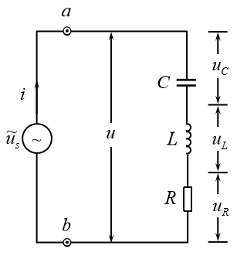
\includegraphics[width=0.3\textwidth]{fig1.png}
    \caption{RLC串联电路图}
    \label{fig:series_circuit}
\end{figure}


\subsubsection{谐振频率与Q值测量}
将电路调整至谐振状态, 确定谐振频率$f_0$. 在该状态下, 使用万用表测量总电压$u$、电感两端电压$u_L$、电容两端电压$u_C$, 并计算品质因数(Q值):
$$
Q = \frac{f_0}{\Delta f} = \frac{u_R}{u - u_R}
$$

\subsubsection{相频特性与幅频特性曲线}
保持总电压$u_{pp}=2.0\,\mathrm{V}$不变, 利用示波器测得电压和电流之间的相位差以及相应的$u_R$. 绘制$\phi-f$曲线和$i-f$曲线, 并估算Q值. 

\subsection{测RLC并联电路的相频特性和幅频特性曲线}

使用如图\ref{fig:parallel_circuit}所示的RLC并联电路, 其中$L=0.1\,\mathrm{H}$, $C=0.05\,\mu \mathrm{F}$, $R'=5\,\mathrm{k}\Omega$. CH1测量总电压, CH2测量$R'$两端电压, 两通道测量电压值相减CH1-CH2即为并联部分的电压$u$. 

\begin{figure}[h]
    \centering
    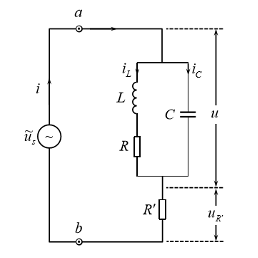
\includegraphics[width=0.3\textwidth]{fig2.png}
    \caption{RLC并联电路图}
    \label{fig:parallel_circuit}
\end{figure}

\subsubsection{谐振频率测量}
调整电路至谐振状态, 找出谐振频率$f_0$. 

\subsubsection{相频特性与幅频特性曲线}
固定总电压$u + u_{R'}$的峰峰值为$2.0\,\mathrm{V}$, 测量并联部分电压$u$(CH1-CH2)与总电流(CH2)的相位差及二者的幅度值. 绘制$\phi-f$曲线和$u-f$、$i-f$曲线. 

\subsection{观测RLC串联电路的暂态过程}

使用如图\ref{fig:transient_circuit}所示的RLC串联电路. 函数发生器产生方波, 设置参数：频率$50\,\mathrm{Hz}$, 电压峰峰值$u_{pp}=2.0\,\mathrm{V}$, 偏移$1\,\mathrm{V}$. 示波器CH1通道测量总电压, CH2测量电容两端电压$u_C$. 实验中$L=0.1\,\mathrm{H}$, $C=0.2\,\mu \mathrm{F}$. 
做如下实验：
\begin{figure}[h]
    \centering
    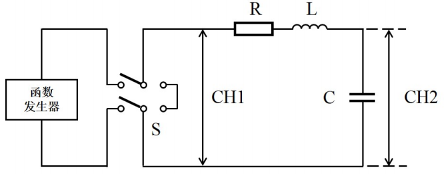
\includegraphics[width=0.5\textwidth]{fig3.png}
    \caption{RLC串联电路暂态过程图}
    \label{fig:transient_circuit}
\end{figure}

\subsubsection{不同电阻值下的暂态响应}
\begin{enumerate}
    \item 当$R=0\,\Omega$时, 测量$u_C$波形. 
    \item 调节$R$以获得临界电阻$R_c$, 并与理论值进行比较. 
    \item 记录$R=2\,\mathrm{k\Omega}$和$R=20\,\mathrm{k\Omega}$时的$u_C$波形. 函数发生器频率分别为$250\,\mathrm{Hz}$($R=2\,\mathrm{k}\Omega$)和$20\,\mathrm{Hz}$($R=20\,\mathrm{k}\Omega$). 
\end{enumerate}

\section{实验数据及处理}
\subsection{RLC串联电路的相频特性和幅频特性曲线}
\begin{table}[H]
\centering
\begin{tabular}{|c|c|c|c|c|} 
\hline
$f/\unit{kHz}$    & $U(V_{\mathrm{pp}})/\unit{V}$ & (CH1-CH2)$\phi/^\circ$  & $U_R(V_{\mathrm{amp}})/\unit{V}$    & $I_{\mathrm{max}}/\unit{mA}$   \\ 
\hline
1.88 & 2 & -86.78  & 0.311 & 1.555  \\ 
\hline
2.00 & 2 & -72.40  & 0.436 & 2.180  \\ 
\hline
2.08 & 2 & -60.86  & 0.571 & 2.855  \\ 
\hline
2.15 & 2 & -41.57  & 0.926 & 4.630  \\ 
\hline
2.19 & 2 & -28.73  & 0.915 & 4.575  \\ 
\hline
2.22 & 2 & -13.32  & 0.956 & 4.780  \\ 
\hline
2.24 & 2 & -3.72   & 0.961 & 4.805  \\ 
\hline
2.25 & 2 & 2.10    & 0.963 & 4.815  \\ 
\hline
2.26 & 2 & 7.00    & 0.958 & 4.790  \\ 
\hline
2.28 & 2 & 16.35   & 0.949 & 4.745  \\ 
\hline
2.30 & 2 & 27.43   & 0.892 & 4.460  \\ 
\hline
2.36 & 2 & 49.20   & 0.743 & 3.715  \\ 
\hline
2.43 & 2 & 57.22   & 0.561 & 2.805  \\ 
\hline
2.62 & 2 & 65.47   & 0.357 & 1.785  \\ 
\hline
3.18 & 2 & 69.94   & 0.187 & 0.935  \\
\hline
\end{tabular}
\caption{RLC串联电路的相频特性和幅频特性数据}
\end{table}

根据在谐振时用万用表测得的电压, 计算品质因素
\begin{equation}
    Q = \dfrac{u_L}{u} = \dfrac{5.35}{0.463} = 11.55
\end{equation}

作$I \sim f$曲线, 如图\ref{fig:series_if}所示.
\begin{figure}[H]
    \centering
    
\includegraphics[width=0.8\textwidth]{plot1.pdf}
    \caption{RLC串联电路的$I \sim f$曲线}
    \label{fig:series_if}
\end{figure}

作$\Delta \phi \sim f$曲线, 如图\ref{fig:series_phi_f}所示.
\begin{figure}[H]
    \centering
    
\includegraphics[width=0.8\textwidth]{plot2.pdf}
    \caption{RLC串联电路的$\Delta \phi \sim f$曲线}
    \label{fig:series_phi_f}
\end{figure}

利用图\ref{fig:series_if}中高斯函数拟合的结果
\begin{equation}
    I(f) = 3.526 \exp \left[- \dfrac{(f - 2.239)^2}{2 \times 0.143^2}\right] + 1.311
\end{equation}
我们得到$I_{\mathrm{max}} = 4.837 \unit{mA}$, $\Delta f = 0.288 \unit{kHz}$, 由此计算得到品质因数
\begin{equation}
    Q = \dfrac{f_0}{\Delta f} = \dfrac{2.239}{0.288} = 7.77
\end{equation}
通过两种方式计算到的品质因素的相对误差是
\begin{equation}
    E_r = \dfrac{11.55 - 7.77}{7.77} \times 100\% = 48.6\%
\end{equation}
两者的相对误差较大, 我们认为后者的结果更为准确.


\subsection{RLC并联电路的相频特性和幅频特性曲线}
\begin{table}[H]
\centering
\begin{tabular}{|c|c|c|c|c|c|c|} 
\hline
$f/\unit{kHz}$    & $U(V_{\mathrm{pp}})/\unit{V}$ & $\Delta t/\unit{\mu s}$&$\phi/^\circ$ & $U$(CH1-CH2)$(V_{\mathrm{amp}})/{\mathrm{V}}$ & $U_R(V_{\mathrm{amp}})/\unit{V}$    & $I_{\mathrm{max}}/\unit{mA}$   \\ 
\hline
2.050 & 2 & -108 & -79.70 & 1.41 & 761  & 0.0761  \\ 
\hline
2.150 & 2 & -94  & -72.76 & 1.61 & 407  & 0.0407  \\ 
\hline
2.220 & 2 & -80  & -63.94 & 1.60 & 239  & 0.0239  \\ 
\hline
2.231 & 2 & -42  & -33.73 & 1.62 & 149  & 0.0149  \\ 
\hline
2.240 & 2 & -24  & -19.35 & 1.63 & 128  & 0.0128  \\ 
\hline
2.247 & 2 & 4    & 3.24   & 1.63 & 118  & 0.0118  \\ 
\hline
2.250 & 2 & 6    & 4.86   & 1.61 & 119  & 0.0119  \\ 
\hline
2.253 & 2 & 12   & 9.73   & 1.60 & 120  & 0.0120  \\ 
\hline
2.256 & 2 & 16   & 12.99  & 1.60 & 123  & 0.0123  \\ 
\hline
2.265 & 2 & 38   & 30.99  & 1.62 & 138  & 0.0138  \\ 
\hline
2.275 & 2 & 52   & 42.59  & 1.58 & 174  & 0.0174  \\ 
\hline
2.320 & 2 & 80   & 66.82  & 1.59 & 342  & 0.0342  \\ 
\hline
2.400 & 2 & 90   & 77.76  & 1.49 & 672  & 0.0672  \\ 
\hline
2.600 & 2 & 92   & 86.11  & 1.18 & 1130 & 0.1130  \\
\hline
\end{tabular}
\caption{RLC并联电路的相频特性和幅频特性数据}
\end{table}

根据表中数据, 分别作$\Delta \phi \sim f$曲线, $U \sim f$曲线和$I \sim f$曲线, 
如图\ref{fig:parallel_phi_f}, \ref{fig:parallel_u_f}, \ref{fig:parallel_i_f}所示.

\begin{figure}[H]
    \centering
    
\includegraphics[width=0.8\textwidth]{plot3.pdf}
    \caption{RLC并联电路的$\Delta \phi \sim f$曲线}
    \label{fig:parallel_phi_f}
\end{figure}

\begin{figure}[H]
    \centering
    
\includegraphics[width=0.8\textwidth]{plot4.pdf}
    \caption{RLC并联电路的$U \sim f$曲线}
    \label{fig:parallel_u_f}
\end{figure}

\begin{figure}[H]
    \centering
    
\includegraphics[width=0.8\textwidth]{plot5.pdf}
    \caption{RLC并联电路的$I \sim f$曲线}
    \label{fig:parallel_i_f}
\end{figure}

可以看到这些曲线和实验原理中的预期是一致的

\subsection{RLC串联电路的暂态过程}
\subsubsection{欠阻尼($R=0\, \Omega,\,f=50\unit{Hz}$)}
\begin{figure}[H]
    \centering
    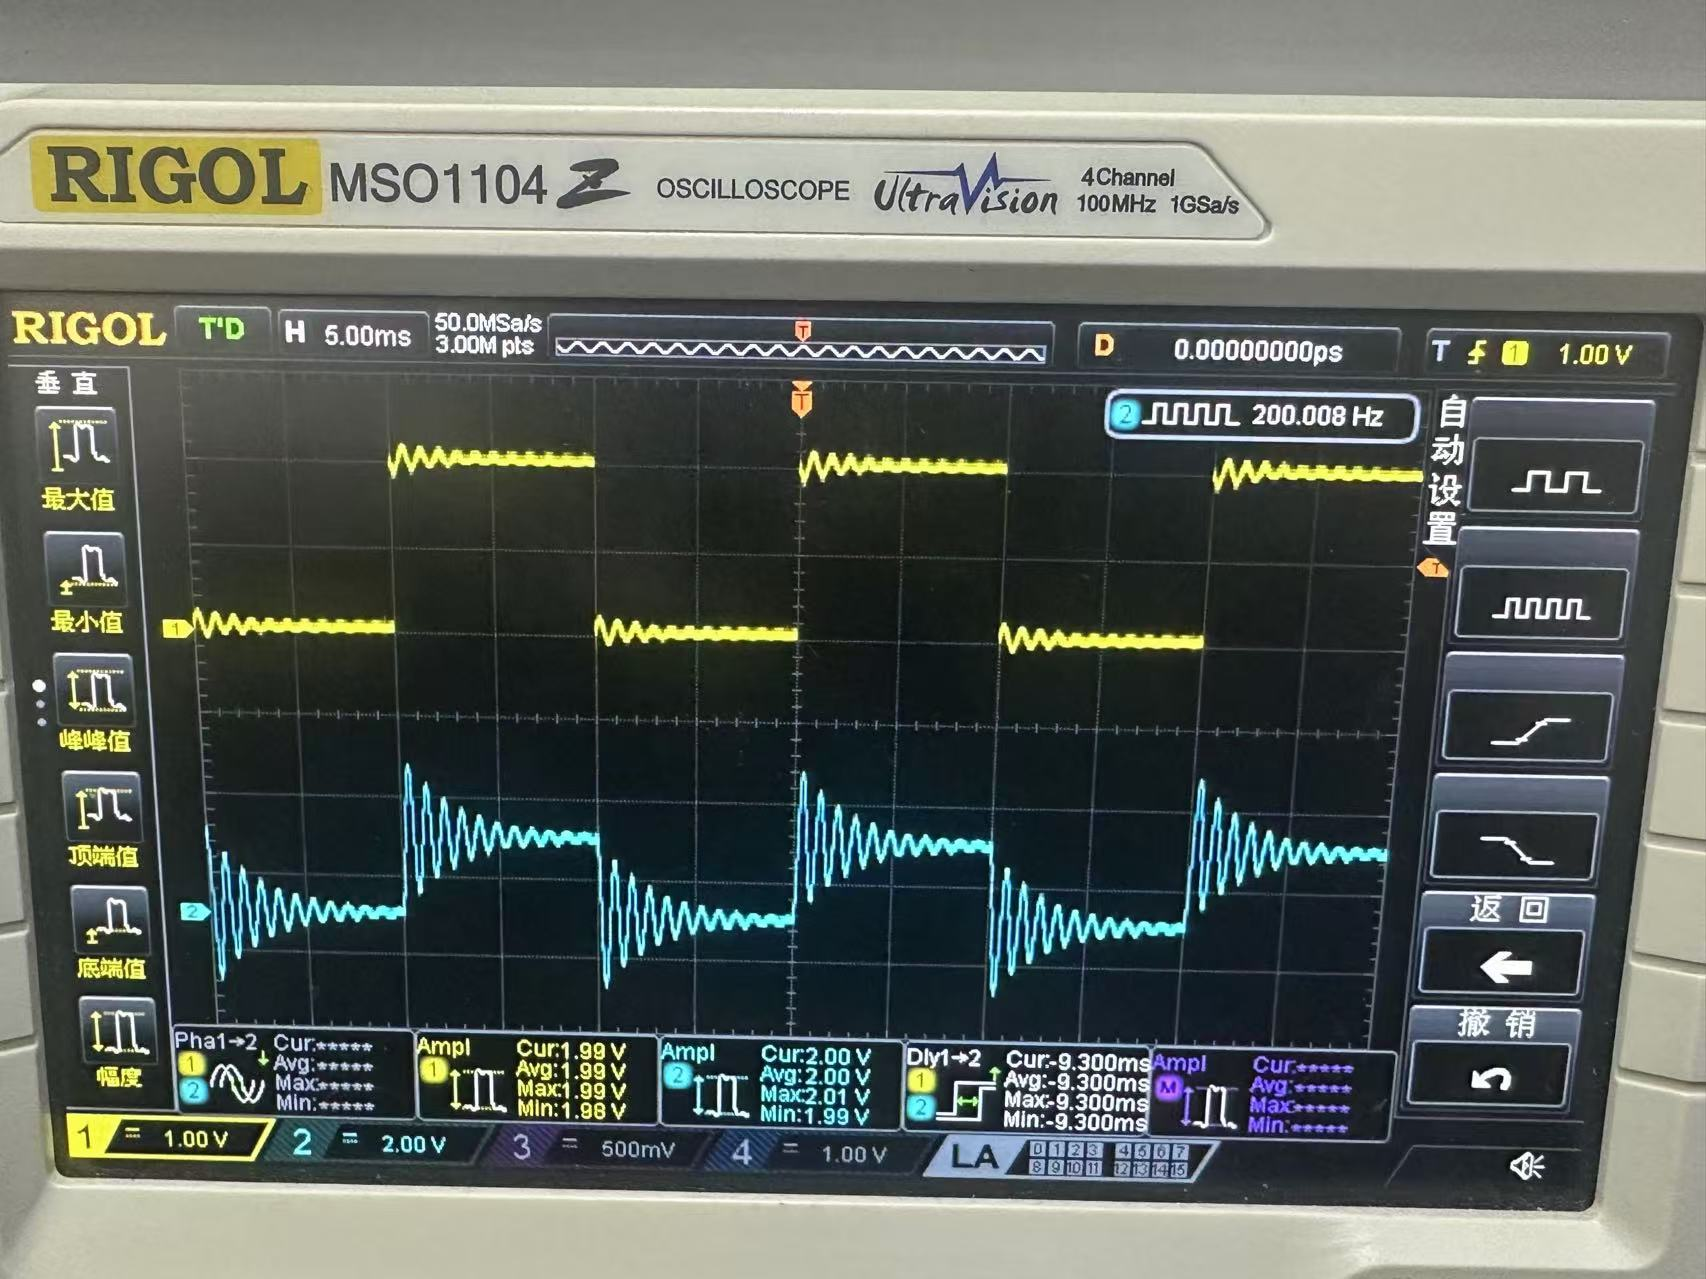
\includegraphics[width=0.7\textwidth]{fig4.jpg}
    \caption{RLC串联电路的暂态过程($R=0,\,f=50\unit{Hz}$)}
    \label{fig:transient_0}
\end{figure}

\subsubsection{临界阻尼($R=1400\, \Omega,\,f=50\unit{Hz}$)}
\begin{figure}[H]
    \centering
    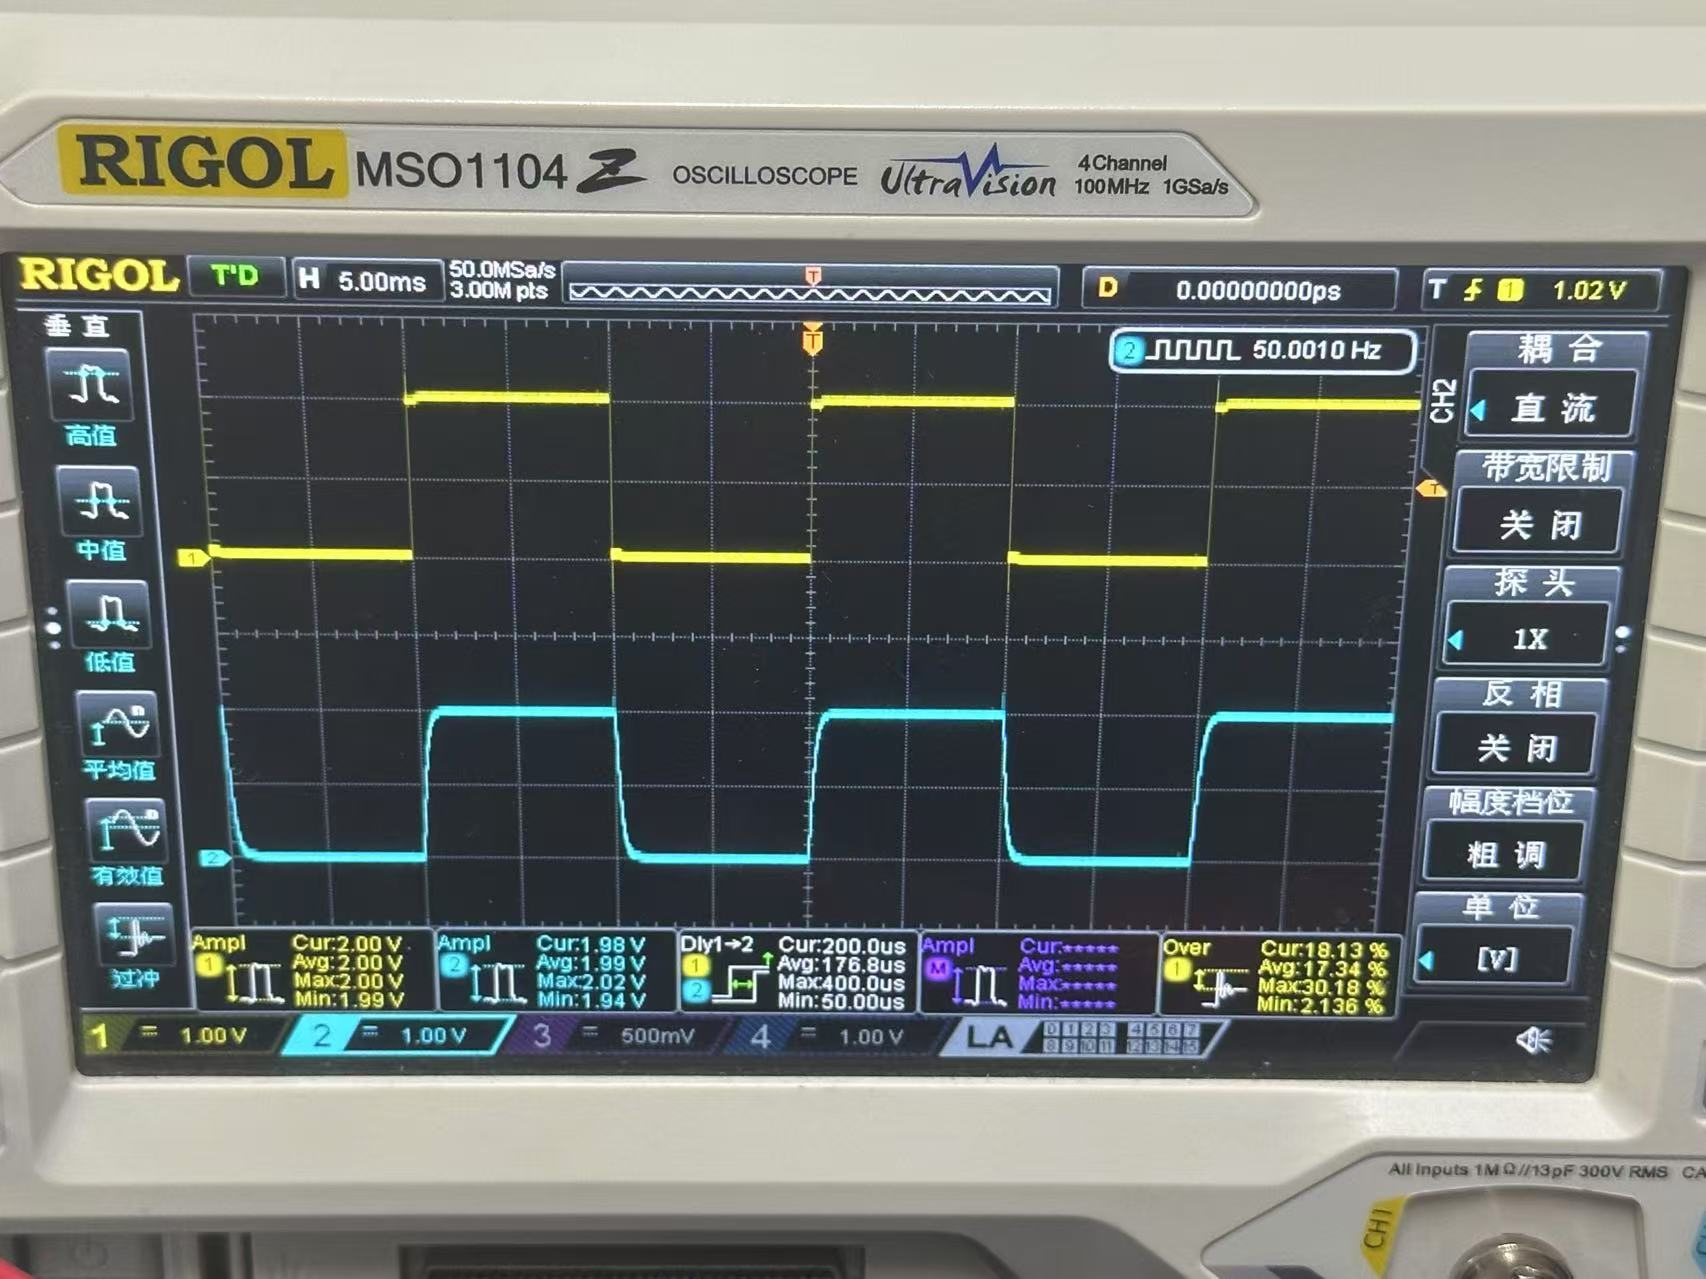
\includegraphics[width=0.7\textwidth]{fig5.jpg}
    \caption{RLC串联电路的暂态过程($R=1400,\,\Omega\,f=50\unit{Hz})$}
    \label{fig:transient_1400}
\end{figure}

实验中达到临界阻尼的电阻值为$R_c' = 1400\,\Omega$(根据示波器测量的过冲百分比最低来判别), 
与理论值$R_c = 1414\,\Omega$相符.

\subsubsection{过阻尼($R=2000\, \Omega,\,f=250\unit{Hz}$)}
\begin{figure}[H]
    \centering
    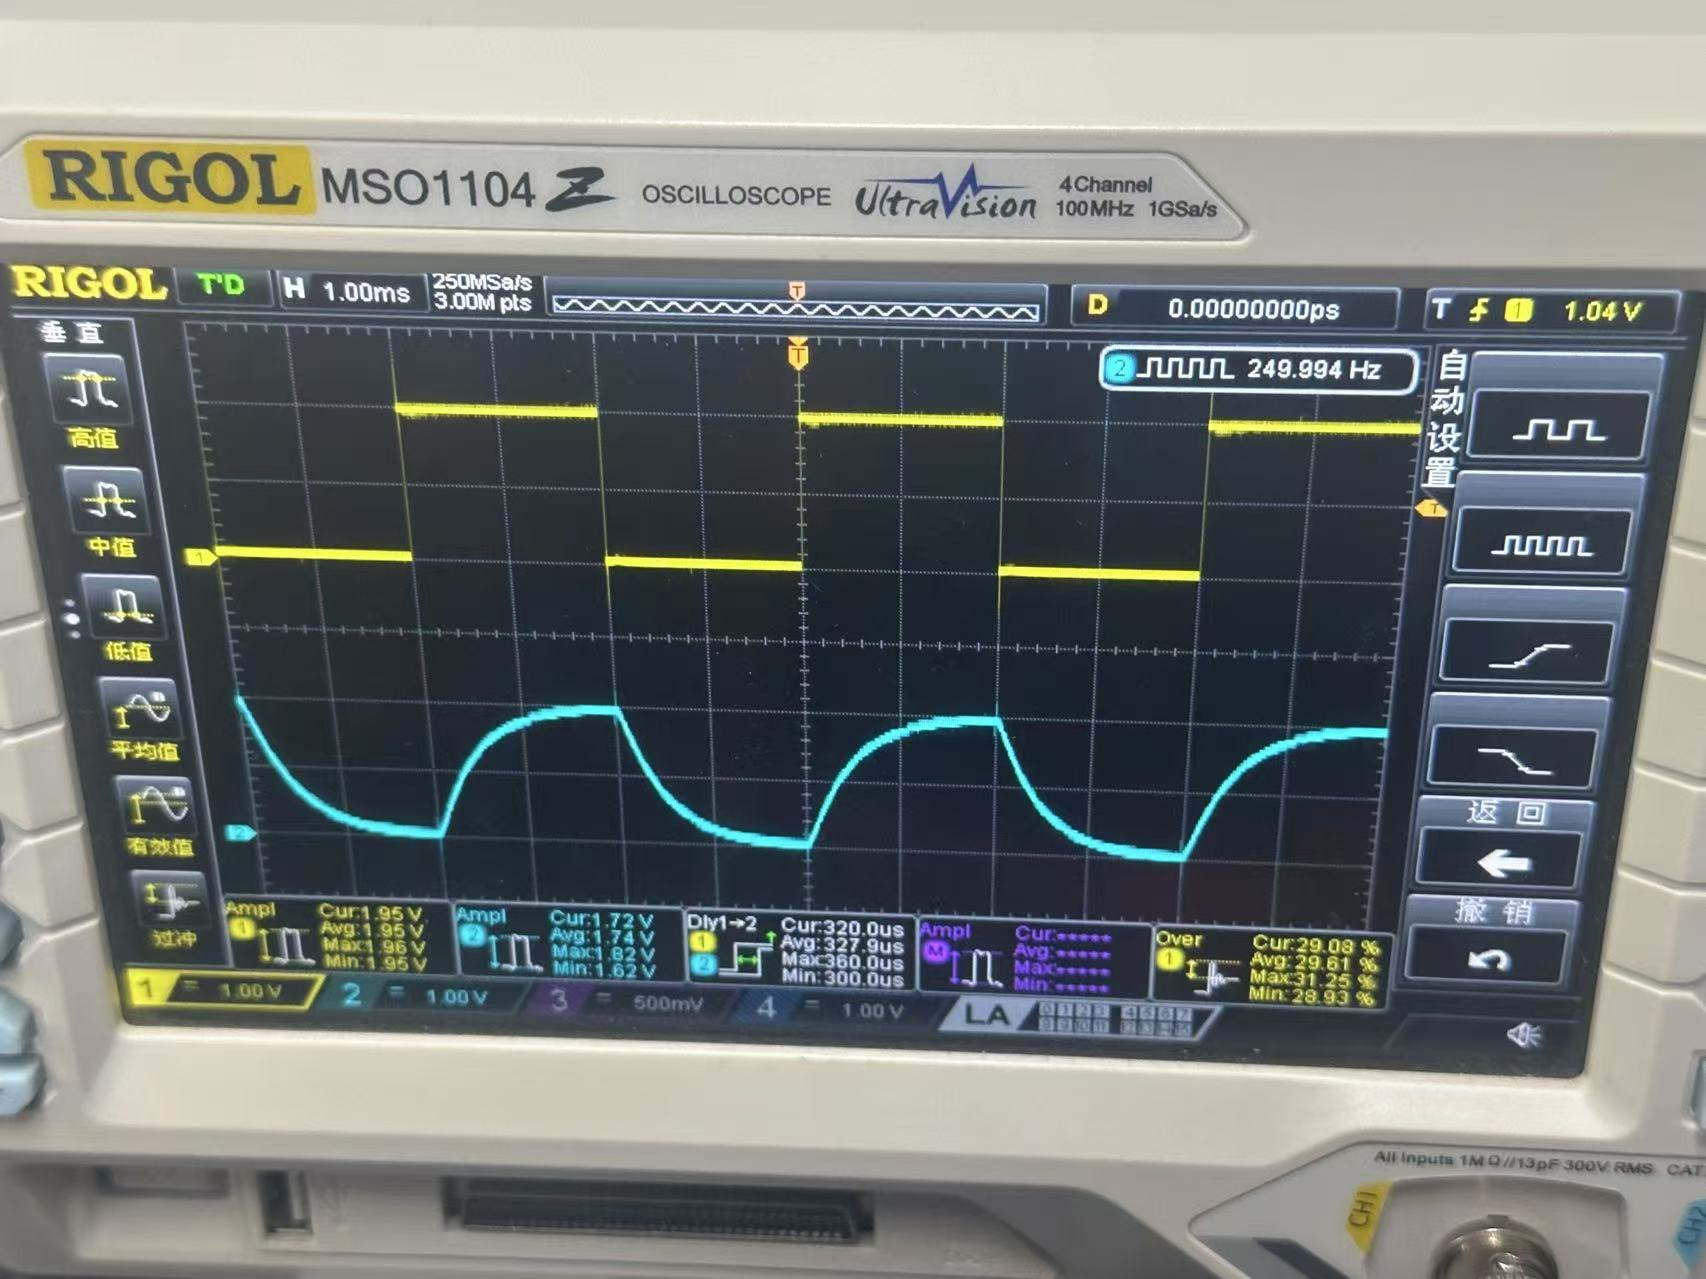
\includegraphics[width=0.7\textwidth]{fig6.jpg}
    \caption{RLC串联电路的暂态过程($R=2000,\,\Omega\,f=250\unit{Hz})$}
    \label{fig:transient_2000}
\end{figure}

\section{实验总结和思考}

本次实验的主要内容是手动连接RLC串联电路和并联电路, 
并用示波器测量电压和电流的相位差和幅度, 来研究RLC电路的谐振现象和阻尼振动规律.
实验整体流程较为简单, 产生的数据也相对较少.

在计算RLC串联电路的品质因素时, 我采用了两种办法: 一种是直接用万用表测量谐振状态时的电压,
通过计算$Q = u_L/u$得到品质因素; 另一种是通过拟合$I \sim f$曲线, 找到曲线的峰值和半高宽,
计算$Q = f_0/\Delta f$. 两种方法得到的结果相差较大. 由于万用表的测量精度较低, 
且实验中使用的万用表在两表头断路的时候也有电压示数, 加之使用万用表时
会使得测量端口处的电路接线更为复杂, 容易引入额外的误差, 所以我认为使用数据拟合的办法
计算到的品质因素更为准确.

在观察RLC并联电路的相频特性和幅频特性曲线时, 需要使用示波器的光标功能测量两个波形之间的时间差,
从而计算出相位差. 但是由于示波器的光标功能的精度较低, 每次移动的都是一个固定的时间间隔,
且我们很难用肉眼准确地确定波峰波谷的位置, 所以这种方法带来的误差较大. 
这个实验中不能像串联情况下那样直接利用示波器的测量功能得到相位差的原因可能是
示波器不支持计算CH1和MATH通道之间的相位差. 为了解决这一点, 我们或许
能够让示波器的两个通道共地直接测量电路的总电压和电容两端的电压, 这样我们就能
够通过示波器直接计算CH1和CH2之间的相位差.

在观察RLC电路的暂态过程时, 很难凭借肉眼确定什么时候达到了临界阻尼的状态, 
这个时候我们可以通过示波器测量过冲的百分比来判断.

\section{附录}

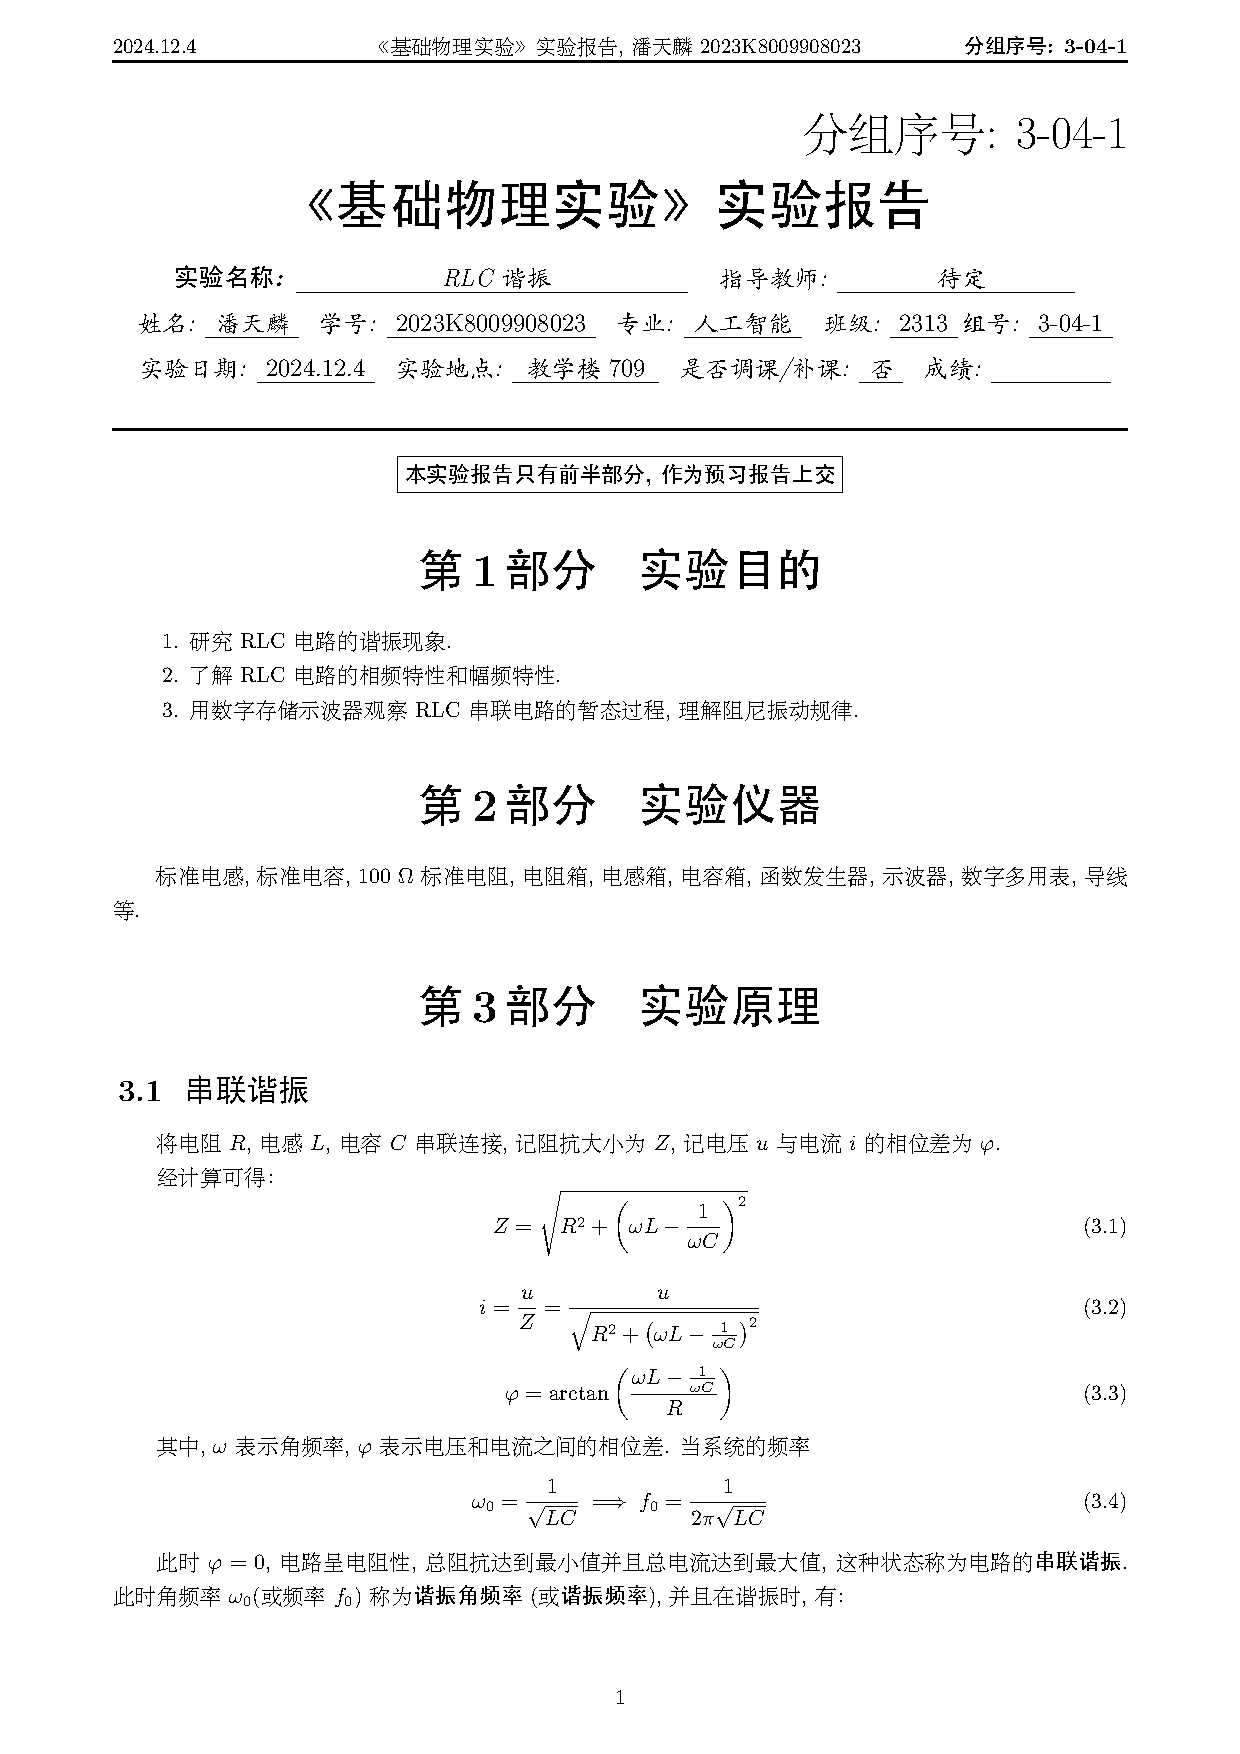
\includepdf[pages=-]{潘天麟-2024-12-4-RLC谐振-预习报告.pdf}
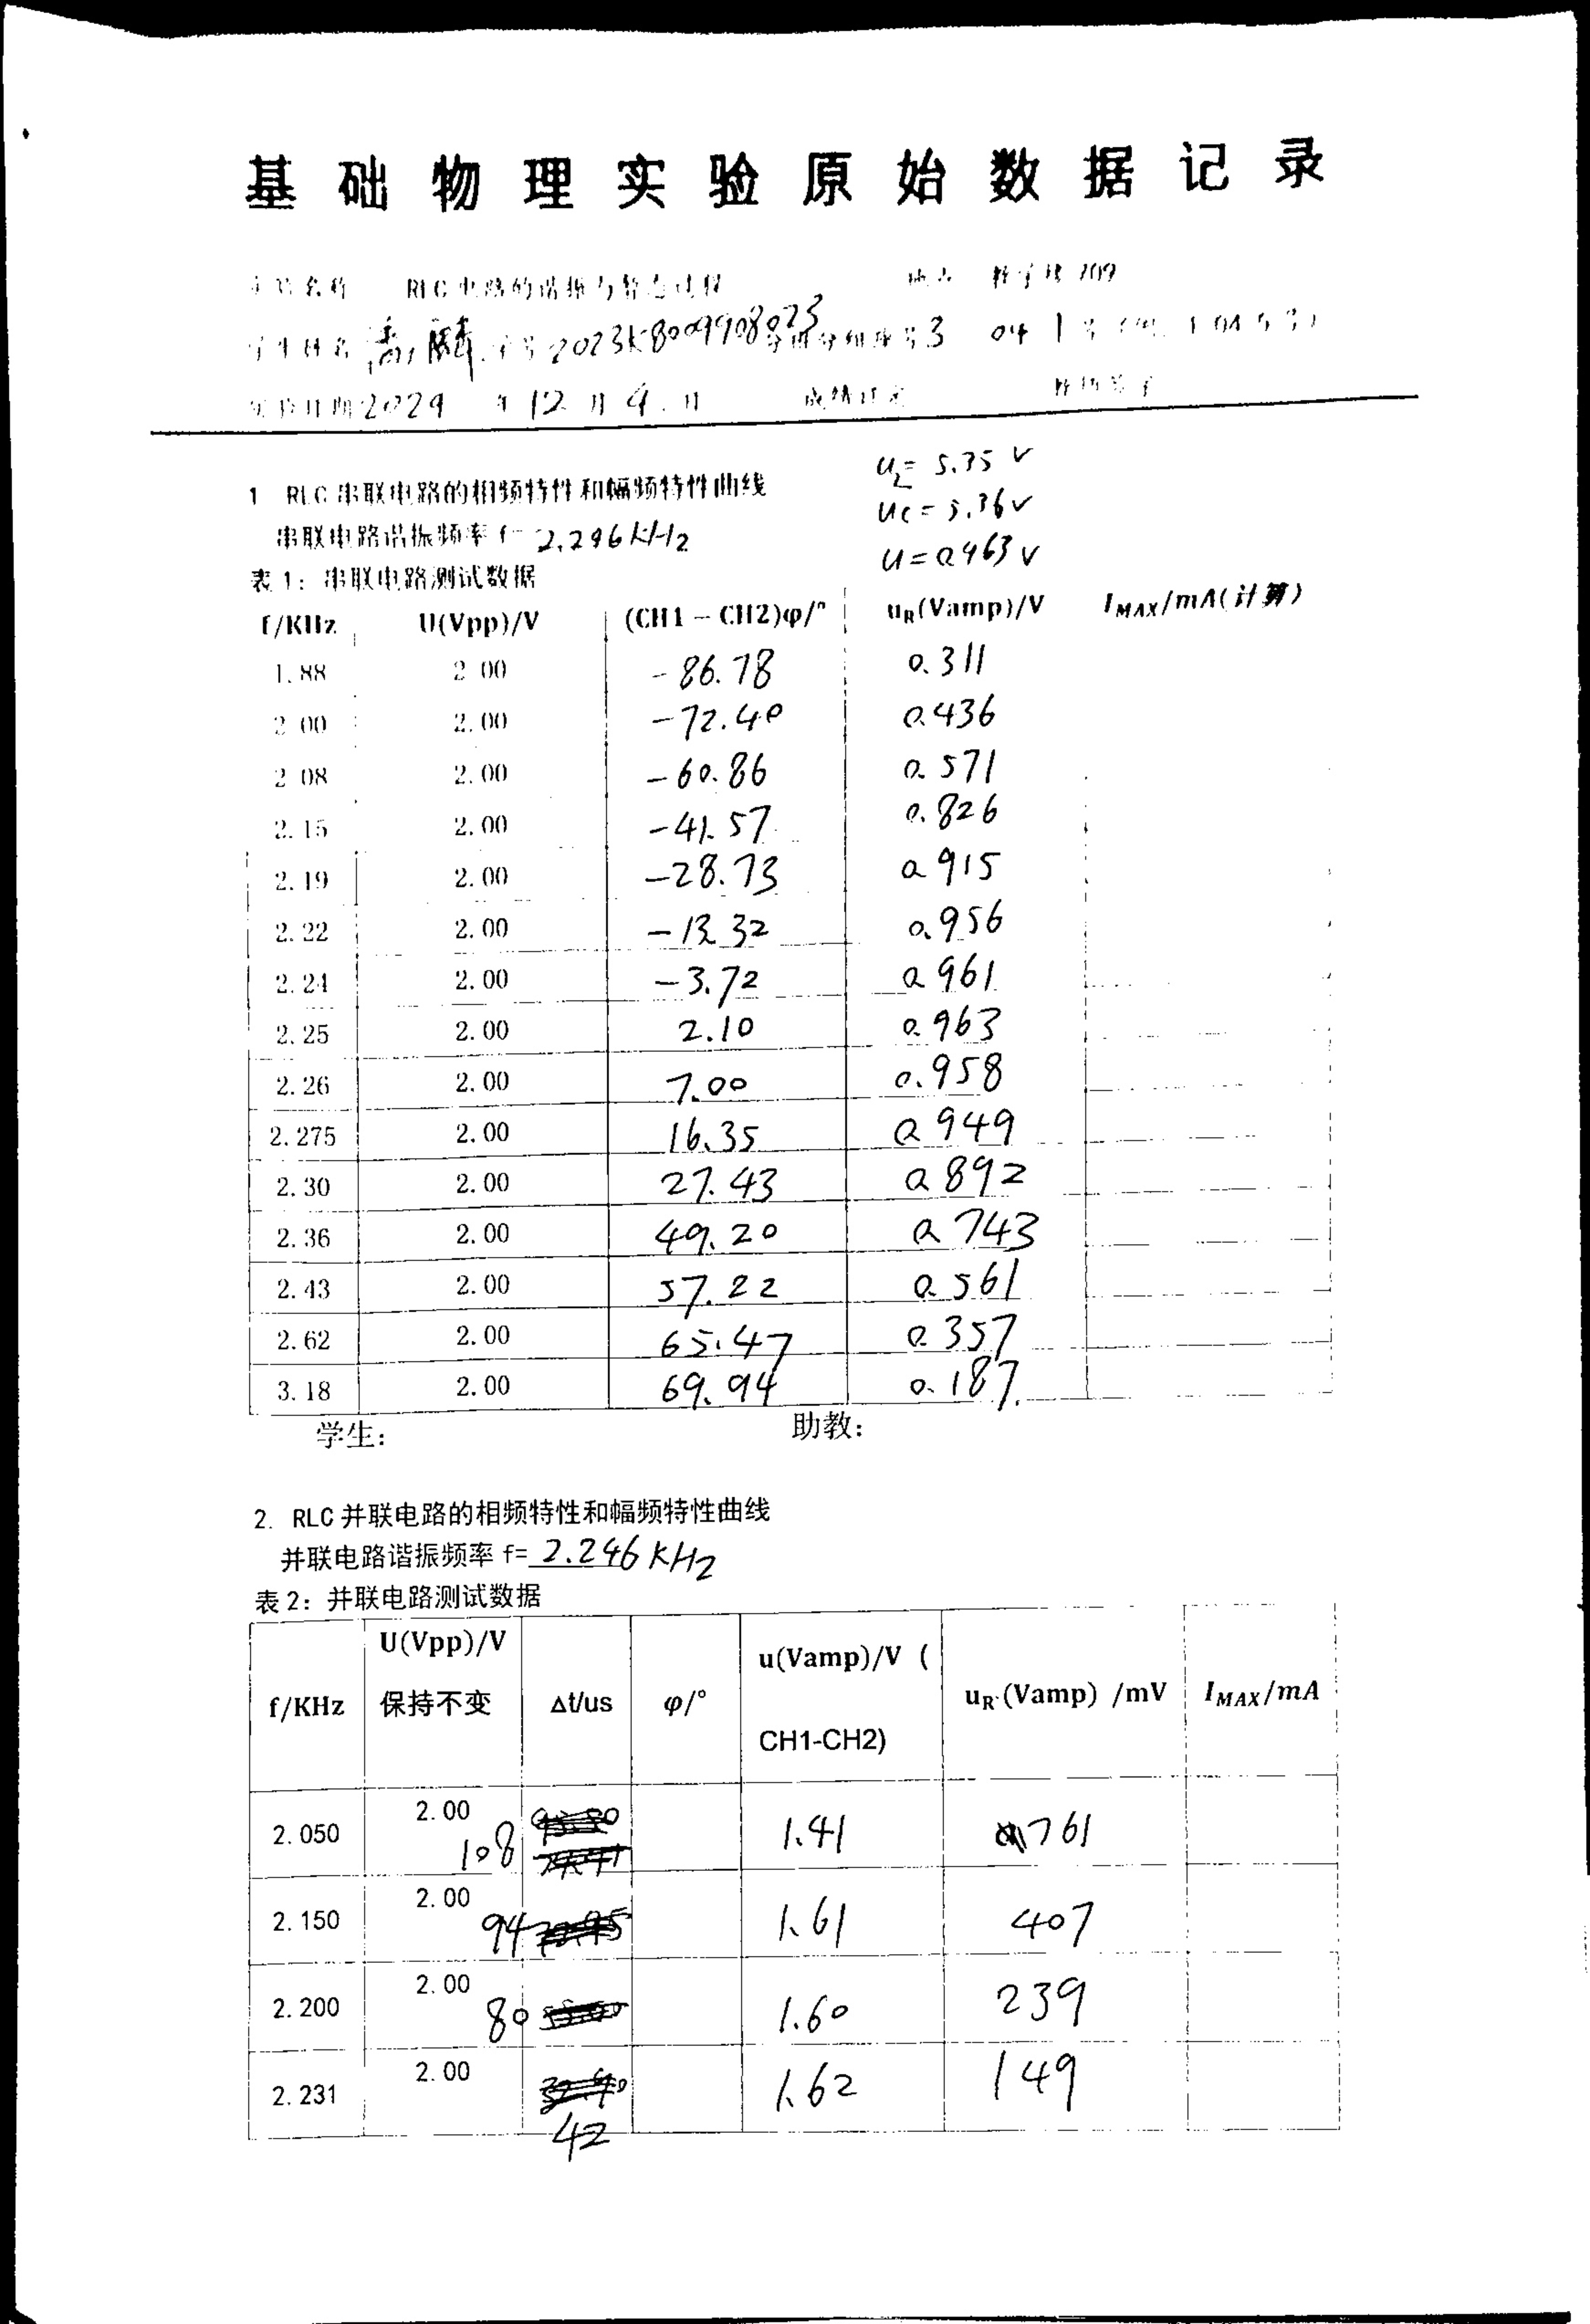
\includepdf[pages=-]{潘天麟-RLC谐振-数据.pdf}

\end{document}

